\documentclass[twocolumn]{article}
\usepackage[margin=1.25in]{geometry}
\usepackage{authblk,setspace}
\usepackage[square,sort,comma,numbers]{natbib}
\usepackage{amsmath,booktabs,array,url,graphicx}
\usepackage[hidelinks]{hyperref}
\usepackage[switch]{lineno}
\setlength{\columnsep}{24pt}
\setstretch{1.15}
\newcommand{\pendingfigure}[2]{%
  \begin{figure*}[t]
    \centering
    \fbox{\begin{minipage}[c][40mm][c]{0.88\textwidth}
      \centering\textbf{Figure pending:} #1\\
      Author-supplied architecture diagram to be inserted.
    \end{minipage}}
    \caption{#2}
  \end{figure*}%
}

\title{MM-Kla: A Target-Aware Multimodal Learning Framework for Protein Lysine Lactylation Site Prediction}
\author[1,$\dag$]{Kaleab Nega}
\author[2,$\dag$]{Zeeshan Abbas}
\author[1,*]{Mobeen Ur Rehman}
\affil[1]{College of Computing and Artificial Intelligence, United Arab Emirates University, Al-Ain 17551, Abu Dhabi, United Arab Emirates}
\affil[2]{Department of Biomedical Engineering, College of IT Convergence, Gachon University, Seongnam, Republic of Korea}
\affil[*]{Correspondence: mobeen.rehman@uaeu.ac.ae}
\affil[$\dag$]{These authors contributed equally to this work.}
\date{}
\begin{document}
\twocolumn[
\begin{@twocolumnfalse}
\maketitle
\begin{abstract}
Protein lysine lactylation (Kla) is a post-translational modification whose
experimental detection requires substantial laboratory effort. Sequence-based
predictors can prioritize candidate sites, but evaluation is sensitive to
repeated windows and related proteins across data partitions. We re-evaluated
MM-Kla on 29,431 accession-verified human Kla candidate sites, partitioned
by protein and screened full-length homology groups into training (20,599),
validation (2,944), and held-out test (5,888). The revised MM-Kla combines a
target-conditioned ProtBERT--descriptor predictor and an independent
position-aware sequence predictor by logistic regression fitted to grouped
out-of-fold scores. On the held-out test, MM-Kla achieved AUPRC 0.8528, AUROC
0.8594, and MCC 0.5507. The matched PCBert-Kla and HybridKla-aligned runs
achieved AUPRC 0.8173 and 0.8454, respectively; a retrained TransKla
implementation reached 0.8555. The gain over the positional predictor alone
was small (AUPRC 0.0048). These are single-seed findings on one balanced
source release. The held-out proteins and screened homology groups are
disjoint, but study-level independence and experimentally verified negative
labels cannot be established from the available records.
\end{abstract}
\noindent\textbf{Keywords:} lysine lactylation; protein language model;
multimodal learning; protein-grouped evaluation; post-translational modification
\vspace{1em}
\end{@twocolumnfalse}
]
\linenumbers

\section{Introduction}
Lysine lactylation was identified as a protein modification connecting
cellular metabolism and gene regulation~\cite{zhang2019metabolic}.
Computational methods can prioritize candidate lysines for validation.
DeepKla introduced a deep-learning predictor for Kla sites, and PCBert-Kla
combined ProtBERT representations with sequence-derived physicochemical
descriptors~\cite{lv2022deepkla,zhang2025pcbert}. HybridKla integrates
multiple sequence and handcrafted-feature predictors; TransKla models local
and global sequence context with cross-attention
~\cite{hybridkla2025,transkla2026}. AttentionKla was introduced with the
human CLEAR-Lactyl dataset~\cite{li2026clear}. DeepPTMPred combines sequence,
protein-language-model, and predicted structural features for several PTM
types, but does not report a Kla predictor~\cite{wang2026deepptmpred}.

The original MM-Kla manuscript used the released DeepKla/PCBert-Kla benchmark.
Audit of its released partitions found 255 of 354 nominal test windows also
present in training, including 170 of 177 positive test windows; four
cross-partition matches had inconsistent labels. The 1,720 positive training
rows represented only 172 distinct windows. These are input-level overlaps,
not merely shared amino-acid motifs. Previous high scores on that nominal
test set therefore cannot substantiate generalization to unseen contexts.
Removing only overlapping test rows would leave just seven positive examples,
which is too few for a stable replacement test estimate. We consequently do
not reuse those scores in the present model ranking.

This revision makes three changes to the evidential basis. First, it constructs
a separate human benchmark with verified accession-position-window identities
and group-disjoint partitions. Second, it evaluates retrained comparators on
the same fixed held-out sites and presents both ranking and threshold-based
metrics. Third, it separates the ProtBERT--descriptor and positional sequence
predictors to test whether their combination contributes beyond either
predictor alone. These changes do not by themselves demonstrate that the
original target-conditioned attention, vector gate, or residual classifier is
individually necessary; that distinction is retained throughout.

\section{Materials and Methods}
\subsection{Experimental Design}
This was a retrospective computational comparison on one public human Kla
release. Site records were cleaned and grouped before model fitting.
Training rows were used to fit model parameters, a disjoint validation
partition was used to compare candidate configurations, and the internal
test was scored after selection. A single predeclared training seed (42)
was available for the reported held-out comparison. The primary ranking
metric was validation AUPRC; all methods were scored on the identical
held-out site list. No published result from a different data partition
was treated as a matched comparator.

\subsection{Source Data and Quality Control}\label{sec:data}
We used the authors' CLEAR-Lactyl release of human candidate Kla sites,
which supplies accessions, residue positions, 51-residue windows, and labels
~\cite{li2026clear}. The source has 33,208 rows, half in each label class.
Each textual \texttt{<pad>} token was normalized to one sequence position
before validation. We retained only canonical, unpadded 51-residue windows
centered on lysine whose accession, position, and sequence exactly matched
the pinned UniProt human reference proteome~\cite{uniprot2025}. Source-labelled negative sites
matching a KlaDB human positive at the same accession-position or at an
identical window were excluded. KlaDB supplied a conflict screen only: it
contributed no training rows and was not used to select models.

The retained dataset has 29,431 unique windows from 4,402 verified proteins:
14,561 labelled positives and 14,870 putative negatives. A negative label
means no Kla annotation in this source, not experimentally verified absence
of Kla. The cleaning process excluded 2,112 padded or noncanonical windows,
166 invalid-length or off-centre windows, 1,218 accessions absent from the
pinned reference, 19 reference mismatches, and 262 negative sites matching
KlaDB positives. These categories and input checksums are recorded in the
preparation audit. No post-split class resampling was applied.

\subsection{Locked Protein-Grouped Split}
Full-length retained proteins were searched against one another with
MMseqs2~\cite{steinegger2017mmseqs2}.
Qualifying hits required at least 30\% sequence identity and 80\% coverage
of both proteins, using sensitivity 7 and E-value 0.001. Connected homology
groups were assigned as units to
training, validation, or held-out test using split seed 42. No accession,
qualifying group, or exact 51-residue window crosses partitions. Table
\ref{tab:split} gives the final counts. This is a protein-grouped internal
test, \emph{not} an experimentally study-disjoint external cohort: the source
does not supply per-site study identifiers, and the screen does not remove
all possible local sequence similarities.
\begin{table*}[t]
\centering
\caption{Locked CLEAR-Lactyl partitions; negative labels are putative.}
\label{tab:split}
\begin{tabular}{lrrrrr}\toprule
Partition & Positive & Negative & Total & Proteins & Groups\\\midrule
Training & 10,191 & 10,408 & 20,599 & 3,037 & 2,480\\
Validation & 1,459 & 1,485 & 2,944 & 442 & 359\\
Held-out test & 2,911 & 2,977 & 5,888 & 923 & 729\\\bottomrule
\end{tabular}
\end{table*}

\subsection{Sequence-Derived Descriptors}
Every site is represented by 27 features calculated from its 51-residue
window: molecular weight, isoelectric point, each of the 20 standard amino
acid fractions, estimated helix/turn/sheet fractions, GRAVY hydropathy, and
charge at pH 7.0. These are sequence-derived \texttt{ProteinAnalysis}
outputs~\cite{cock2009biopython}, not experimental physicochemical
measurements or structural data.
The code and exact feature order are released with the implementation.
The helix/turn/sheet outputs are composition-based estimates, not measured
secondary structure. Min--max scaling is fit only on the fitting subset and applied
unchanged to validation and held-out rows.

The ProtBERT predictor also uses CKSAAP frequencies for ordered residue
pairs with gaps $k\in\{0,1,2,3\}$. The frequency of each pair is its
count divided by $50-k$ for a 51-residue window, giving $4\times20^2=1,600$
additional features. Thus its descriptor vector has 1,627 components.
Within each fitting fold, scaling parameters are learned from that fold's
training rows only.

\begin{table*}[t]
\centering
\caption{Exact order of the 27 sequence-derived descriptors. All are
computed from the 51-residue window with Biopython
\texttt{ProteinAnalysis}. The implementation version must be reported
from the frozen training environment before submission.}
\label{tab:features}
\small
\begin{tabular}{@{}p{0.08\textwidth}p{0.42\textwidth}p{0.42\textwidth}@{}}\toprule
Index & Descriptor(s) & Implementation call or definition\\\midrule
1 & Molecular weight & \texttt{molecular\_weight()}\\
2 & Isoelectric point & \texttt{isoelectric\_point()}\\
3--22 & Fractions of A, C, D, E, F, G, H, I, K, L, M, N, P, Q, R, S, T, V, W, Y &
  Residue count divided by 51\\
23--25 & Helix, turn, sheet fractions & \texttt{secondary\_structure\_fraction()}\\
26 & GRAVY hydropathy & \texttt{gravy()}\\
27 & Net charge at pH 7.0 & \texttt{charge\_at\_pH(7.0)}\\\bottomrule
\end{tabular}
\end{table*}

\subsection{Two-Predictor MM-Kla}\label{sec:model}
The first predictor fine-tunes the first four encoder layers of
\texttt{Rostlab/prot\_bert}. A central-lysine embedding conditions additive
attention over valid residue embeddings. If $h_K$ is the central embedding,
the scores, normalized weights, and pooled sequence vector are
\begin{align}
e_i &= v^\top\tanh(W_t h_i+W_K h_K+b),\\
\alpha_i &= \frac{m_i\exp(e_i)}{\sum_j m_j\exp(e_j)},\qquad
h_{\mathrm{seq}}=\sum_i\alpha_i h_i,
\end{align}
where $m_i$ excludes padding and special tokens. The pooled vector and the
scaled descriptor vector are projected to 256 dimensions. A vector-valued,
sample-dependent gate fuses them:
\begin{equation}
\begin{aligned}
g&=\sigma\left(W_g[z_{\mathrm{seq}};z_{\mathrm{feat}}]+b_g\right),\\
z&=g\odot z_{\mathrm{seq}}+(1-g)\odot z_{\mathrm{feat}}.
\end{aligned}
\end{equation}
Two residual multilayer-perceptron blocks and a sigmoid output yield
the first Kla score. Attention and fusion dimensions are 256; dropout is
0.2. The second predictor uses only the sequence: learned 64-dimensional
residue and position embeddings feed a two-layer bidirectional LSTM with
64 hidden units per direction. Central-state-conditioned attention pools
the LSTM outputs, and a small classifier produces a separate Kla score.

Five stratified, homology-grouped outer folds generate out-of-fold scores
for both predictors on the training partition. Within each outer fold,
training duration is selected on an inner grouped split; the selected
models are refit on the outer training rows before scoring the outer-held
rows. A logistic regression combiner ($C=1$) is trained on the resulting
two-score out-of-fold pairs. Each predictor's score on validation or test
is averaged over its five outer-fold models before applying the fixed
combiner. Both individual predictors and an unweighted score average are
retained as controls. Neither the combiner nor any fold model is trained
on held-out test labels.

\pendingfigure{Two-predictor architecture and grouped stacking flow}
{Revised MM-Kla: ProtBERT--descriptor and positional sequence predictors
generate independent scores. A logistic combiner is fitted on grouped
out-of-fold training scores only.\label{fig:framework}}

\subsection{Training, Selection, and Evaluation}
The ProtBERT predictor uses AdamW, encoder learning rate $2\times10^{-5}$,
head learning rate $10^{-4}$, weight decay 0.01, batch size four, and a
linear schedule with 10\% warm-up. The positional predictor uses AdamW,
learning rate $10^{-3}$, weight decay 0.01, and batch size 128. Both use
unweighted binary cross-entropy and at most 30 epochs; inner selection is
by AUPRC with patience five. Validation AUPRC is the primary criterion
for selecting the candidate configuration. The held-out partition is
reserved for final scoring. We report AUPRC, AUROC, MCC, F1, precision,
recall, specificity, and accuracy. Unless a development-only threshold
is explicitly declared, threshold-dependent metrics use 0.5. The
positive class is Kla.

\subsection{Statistical Analysis}
AUPRC is average precision over the ranked scores;
AUROC is the area under the receiver operating characteristic curve.
The test set was not used for threshold or architecture selection.
We resampled the 729 held-out homology groups with replacement 2,000 times,
recomputing paired AUPRC differences for each resample. Percentile limits
are descriptive conditional intervals for these trained models, not
uncertainty over independent retraining seeds or laboratories.

\subsection{AI-Assisted Preparation}
OpenAI Codex was used for drafting and checking analysis code and text.
All numerical results reported here were recomputed from saved per-site
predictions, not generated by a language model. \textbf{[Before submission,
identify the exact tool/model version and provide the complete prompts
used in producing this work, as required by the journal.]}

\subsection{Comparators}
PCBert-Kla, HybridKla architecture-aligned, DeepKla architecture-aligned,
and TransKla were evaluated on the same locked partitions
~\cite{zhang2025pcbert,hybridkla2025,lv2022deepkla,transkla2026}.
The PCBert-Kla implementation used the first four ProtBERT layers, the 27
descriptors, AdamW at $2\times10^{-5}$, batch size four, and validation AUPRC
for early stopping (selected epoch four). The original token-gated MM-Kla
configuration was evaluated as another control (selected epoch three).
The DeepKla-aligned predictor was selected at epoch nine. The HybridKla-
aligned implementation trained an ESM2-150M branch, an LSTM branch, and six
handcrafted feature-family predictors with five grouped folds and a meta
classifier; its stacking protocol differs from the original authors'
pipeline. The TransKla implementation was retrained on the locked
partitions and selected at epoch 14 by validation AUPRC. Thus the
\emph{data rows and evaluation metrics} are matched, but model-specific
training protocols and feature families are not identical. ``Aligned''
models are not claimed as exact reproductions of their authors' full
implementations. Published scores from unrelated benchmarks are excluded.
DeepPTMPred is discussed as related PTM work rather than a Kla comparator
because its released tasks do not include Kla~\cite{wang2026deepptmpred}.

\section{Results}
\subsection{Matched Held-Out Evaluation}
All predictions in Table~\ref{tab:performance} were aligned by accession,
one-based site position, and reference label to the locked test manifest
before metrics were recomputed. All 5,888 scores per model were finite and
within $[0,1]$. The held-out Kla prevalence was 2,911/5,888 (49.4\%).
MM-Kla's two-predictor combination reached AUPRC 0.8528, compared with
0.8173 for PCBert-Kla and 0.8454 for HybridKla-aligned. The retrained
TransKla implementation had the highest observed AUPRC (0.8555), AUROC
(0.8683), MCC (0.5697), and accuracy (0.7845) among these runs. MM-Kla
therefore does not lead the complete matched comparison.
\begin{table*}[t]
\centering
\caption{Matched CLEAR-Lactyl internal held-out performance on the same
5,888 sites (seed 42). AUPRC denotes average precision. Threshold-dependent
metrics use 0.5. ``Aligned'' denotes an implementation adapted to this
benchmark rather than exact reproduction of the original pipeline.}
\label{tab:performance}
\small
\begin{tabular}{lrrrrrrrr}\toprule
Method & AUPRC & AUROC & MCC & F1 & Pre & Rec & SP & ACC\\\midrule
PCBert-Kla & 0.817 & 0.828 & 0.487 & 0.761 & 0.689 & 0.849 & 0.626 & 0.736\\
DeepKla-aligned & 0.815 & 0.820 & 0.466 & 0.724 & 0.741 & 0.708 & 0.757 & 0.733\\
HybridKla-aligned & 0.845 & 0.855 & 0.539 & 0.771 & 0.759 & 0.783 & 0.756 & 0.770\\
TransKla & 0.856 & 0.868 & 0.570 & 0.787 & 0.770 & 0.804 & 0.765 & 0.784\\
MM-Kla (original token gate) & 0.813 & 0.826 & 0.489 & 0.752 & 0.720 & 0.787 & 0.700 & 0.743\\
MM-Kla (ProtBERT branch) & 0.825 & 0.831 & 0.482 & 0.734 & 0.746 & 0.723 & 0.759 & 0.741\\
MM-Kla (positional branch) & 0.848 & 0.856 & 0.546 & 0.772 & 0.767 & 0.776 & 0.770 & 0.773\\
MM-Kla (two-predictor) & 0.853 & 0.859 & 0.551 & 0.776 & 0.764 & 0.789 & 0.762 & 0.775\\
\bottomrule\end{tabular}

\end{table*}

Figure~\ref{fig:curves} displays the threshold-independent comparison.
At a threshold of 0.5, MM-Kla correctly identified 2,297 positive sites,
missed 614, and made 710 false-positive calls. TransKla identified 2,341
positives, missed 570, and made 699 false-positive calls
(Fig.~\ref{fig:confusion}). These counts explain the threshold-dependent
margin without relying on accuracy alone.
\begin{figure*}[t]
\centering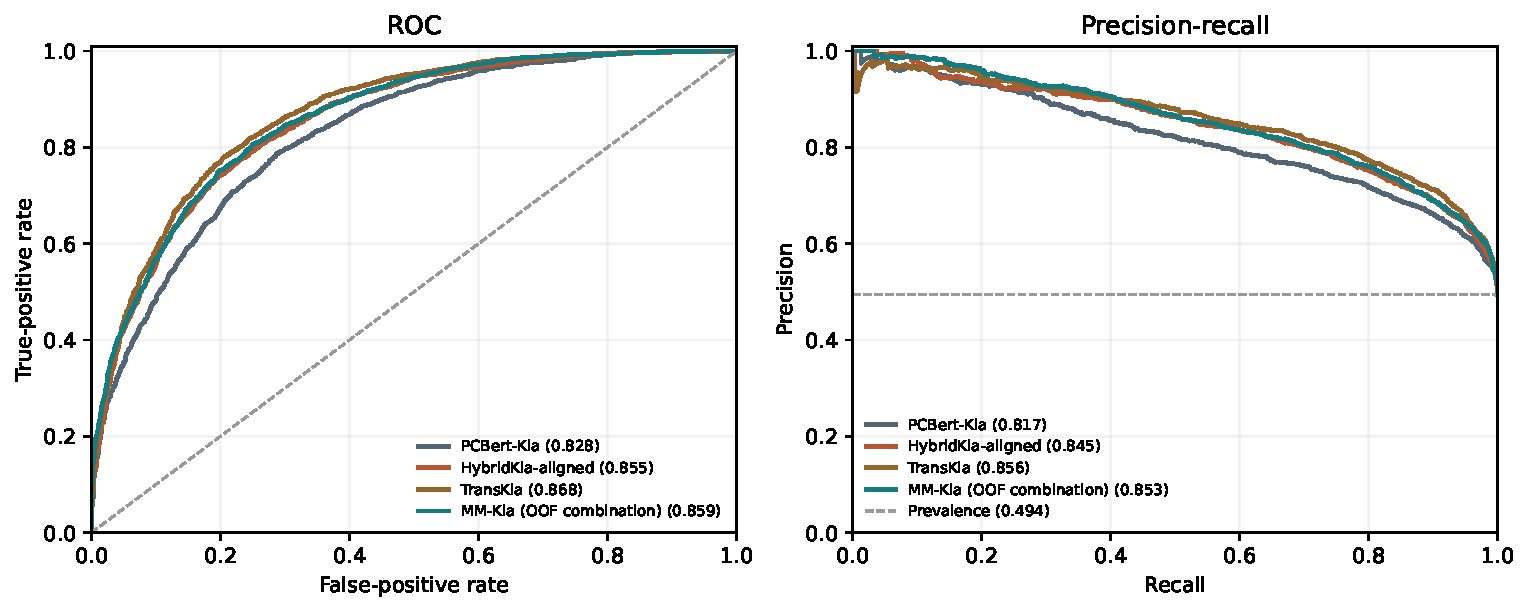
\includegraphics[width=0.92\textwidth]{figures_generated/heldout_curves.pdf}
\caption{Held-out ROC and precision--recall curves from the same labelled
5,888 sites. Legend values are AUROC and AUPRC, respectively; the dashed
precision line denotes test prevalence. Curves do not include training-seed
uncertainty.}\label{fig:curves}
\end{figure*}
\begin{figure*}[t]
\centering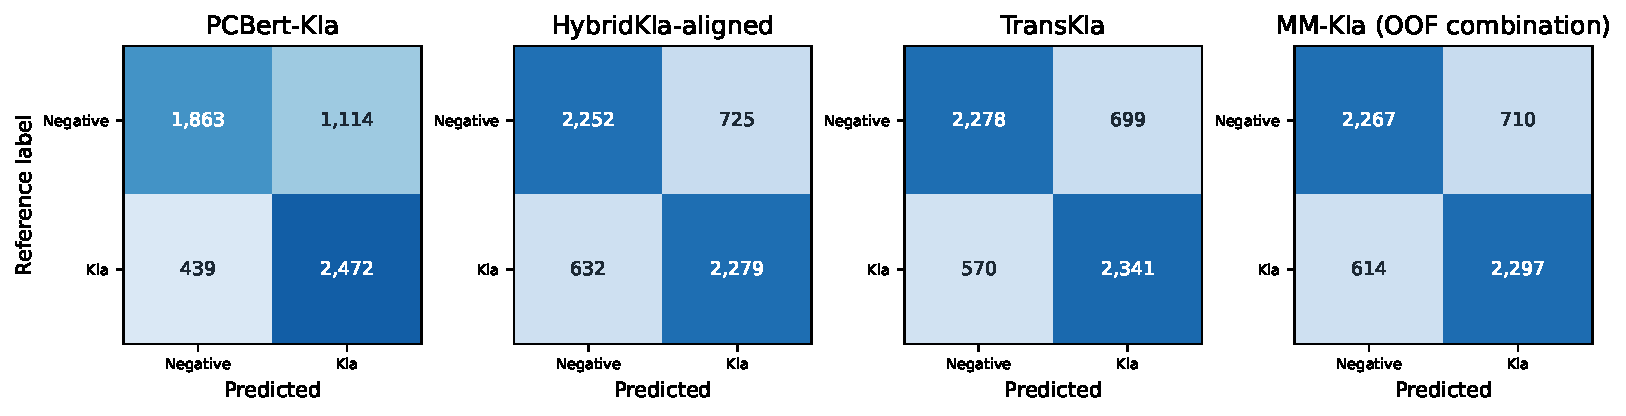
\includegraphics[width=0.95\textwidth]{figures_generated/confusion_matrices.pdf}
\caption{Confusion matrices on the held-out internal test at the fixed 0.5
decision threshold. Rows are reference labels and columns are predictions.}
\label{fig:confusion}
\end{figure*}

\subsection{Paired Uncertainty on the Held-Out Proteins}
The observed MM-Kla minus PCBert-Kla AUPRC difference was 0.0355; the
paired homology-group bootstrap yielded a descriptive 95\% interval of
[0.0278, 0.0432]. The difference against HybridKla-aligned was 0.0075
[0.0030, 0.0124]. Against TransKla, the difference was $-0.0027$
[$-0.0159$, 0.0101], consistent with either ordering under resampling of
the held-out groups. These intervals condition on one training seed and
one source cohort. They do not resolve retraining variability or selection
effects from using the common validation set.

\subsection{Predictor Contributions and Remaining Ablations}
The held-out ProtBERT--descriptor predictor achieved AUPRC 0.8246 and the
positional predictor achieved 0.8481. Their unweighted score average
reached 0.8512; the grouped out-of-fold logistic combination reached
0.8528 (Fig.~\ref{fig:components}). The combination's improvement over
the stronger individual predictor was 0.0048 AUPRC, with paired
group-resampling limits [0.0011, 0.0083] for the saved seed-42 models.
The corresponding validation AUPRC values were 0.8244, 0.8584, 0.8570,
and 0.8598. Thus the validation ranking of the two-predictor combination
was broadly retained, but the incremental gain is small. A strong
positional branch accounts for most of its performance.

This predictor-level control does not isolate the vector gate from the
ProtBERT input, the 27 descriptors from CKSAAP, or the residual classifier
from the head. The present single-run benchmark does not include matched
CLS/mean/max pooling, scalar-gate/concatenation, no-residual, or
frozen-versus-fine-tuned controls on the locked split. Claims that those
specific components independently cause the observed improvement are
therefore not supported. The original token-gated configuration, without
the added CKSAAP and positional predictor, reached AUPRC 0.8134 on the
same held-out set, below PCBert-Kla's 0.8173; the revised model changes
several factors simultaneously, so its gain cannot be assigned to one.
\begin{figure}[t]
\centering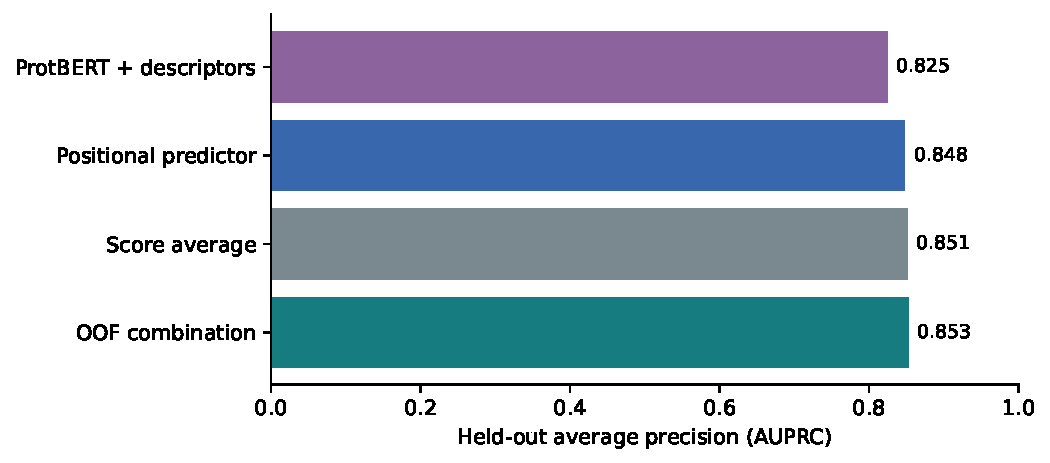
\includegraphics[width=\columnwidth]{figures_generated/component_scores.pdf}
\caption{Predictor-level comparison for the revised MM-Kla on the
held-out internal test. This is not a module-level ablation of attention,
gating, or residual layers.}\label{fig:components}
\end{figure}

\subsection{Exploratory Encoder-Depth Check}
Development runs on the same locked training and validation partitions
provide a limited check of the four-layer truncation (Table~\ref{tab:depth}).
The four-layer token-gated model reached validation AUPRC 0.8198; using
all 30 ProtBERT layers with all layers trainable reached 0.7523, while
using all 30 layers with only the last four trainable reached 0.6960.
These single-seed runs used AdamW, batch size four, and a 30-epoch cap,
with validation-based early stopping. The result does not establish that
four layers is optimal: intermediate depths, repeated seeds, matched
compute budgets, and parameter/memory measurements are still needed.
\begin{table}[t]
\centering
\caption{Exploratory ProtBERT depth configurations on the locked
validation partition (seed 42, token-gated head). These are development
results, not held-out test scores or a complete depth sweep.}
\label{tab:depth}
\small
\setlength{\tabcolsep}{4pt}
\begin{tabular}{lrrr}\toprule
Encoder & Trainable & Epoch & AUPRC\\\midrule
First 4 layers & 4 & 3 & 0.8198\\
All 30 layers & 30 & 2 & 0.7523\\
All 30 layers & Last 4 & 2 & 0.6960\\\bottomrule
\end{tabular}
\end{table}

\subsection{Sequence-Context Description}
Figure~\ref{fig:context} shows the observed difference in amino-acid
frequency at each position in the held-out 51-residue windows, positive
minus putative-negative. It is computed directly from the 2,911 and 2,977
reference-labelled sites, respectively, with no model scores. This figure
identifies compositional contrasts around candidate lysines but does not
show a causal motif, validate a binding mechanism, or prove that the
attention mechanism uses those residues. Because multiple sites can come
from a protein and negatives are putative, individual cells are not given
independent-site significance labels. The original attention-profile and
t-SNE plots were not reused: their old data partition was contaminated
by exact-window overlap, and average attention is not a faithfulness test.
\begin{figure*}[t]
\centering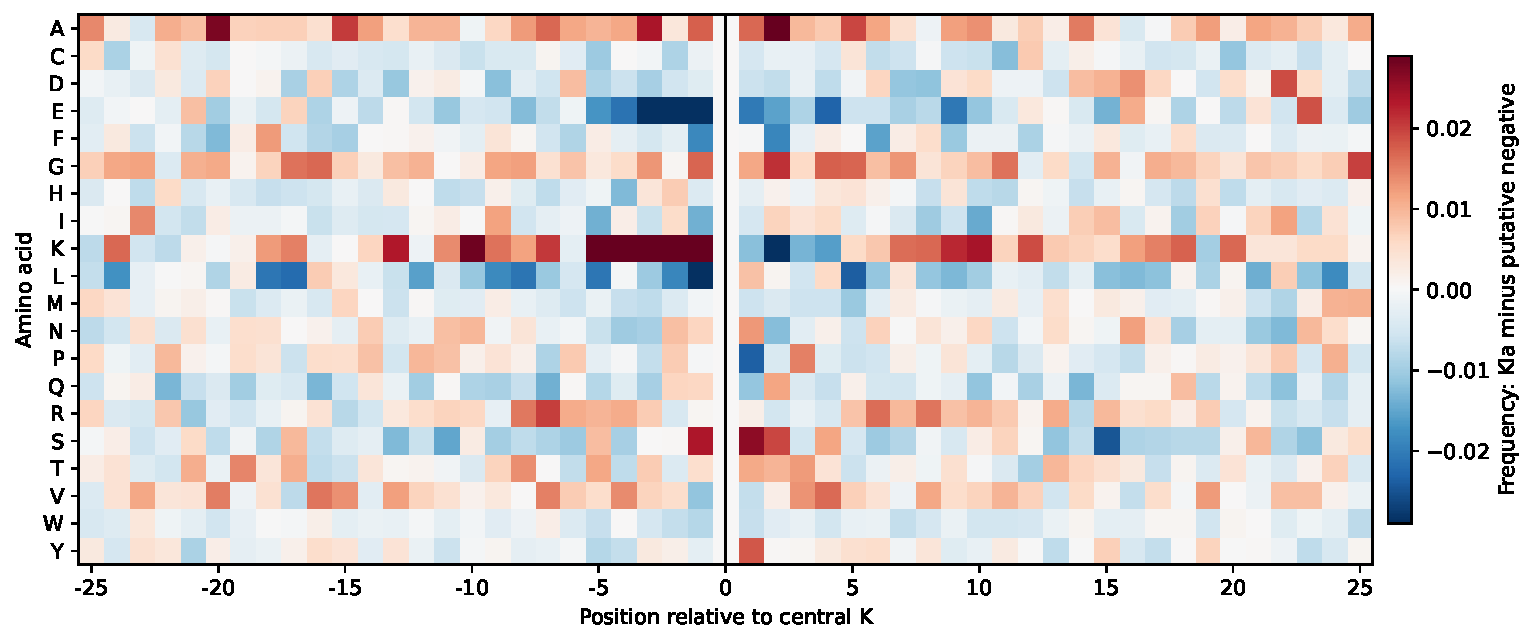
\includegraphics[width=0.92\textwidth]{figures_generated/sequence_context.pdf}
\caption{Position-wise amino-acid frequency difference on the locked
held-out internal test (Kla minus putative negative). The central lysine
at position zero is fixed by construction; color values are descriptive
frequency differences, without per-cell significance testing.}
\label{fig:context}
\end{figure*}

\section{Discussion}
The original benchmark leakage changed the interpretation of the entire
study: a strong result on overlapping windows was not evidence that MM-Kla
would generalize to unseen proteins. The accession-checked CLEAR-Lactyl
split resolves exact-window overlap and screens related full-length
proteins before assigning partitions. This makes the present internal test
more informative than the earlier nominal independent test. It does not
turn a single-source split into a separately collected external cohort.

The two-predictor MM-Kla improved AUPRC over PCBert-Kla and the adapted
HybridKla comparison in this run, but TransKla was numerically ahead.
The increase from the positional predictor alone was small. It is more
accurate to describe this as evidence that the two predictors are somewhat
complementary under the present training protocol than as proof that the
physicochemical gate is necessary. The strongest component-level claim
remaining from the original manuscript requires its own matched ablations.

Four limitations constrain the conclusions. First, source site records
lack per-study identifiers, so study-level independence is unverified;
the homology rule also does not exclude every shared local domain or motif.
Second, negative labels represent unreported sites rather than measured
non-lactylation. Third, near-equal class prevalence in the test set differs
from prospective proteome screening, where a far lower prior prevalence
would reduce precision at a fixed sensitivity. Fourth, the present
held-out comparison uses one trained seed; paired group bootstrap does not
substitute for independent training repeats. Further work should provide
a cross-source cohort screened against the training proteins, repeated
seeds, direct component ablations, and residue-perturbation experiments.
These are outstanding validation requirements, not completed analyses.

\subsection{Conclusions}
The revised two-predictor MM-Kla reached AUPRC 0.8528 on the locked
protein/homology-group-held-out CLEAR-Lactyl split, above the matched
PCBert-Kla and HybridKla-aligned runs but below TransKla. Most of the
MM-Kla performance came from its position-aware sequence predictor.
The revised benchmark supports a bounded claim about generalization to
unseen proteins and screened homology groups within this source release;
broader generalization and the necessity of individual architectural
components remain open.

\section*{Data and Code Availability}
Source code, split-construction scripts, and the per-site held-out
prediction files used for the tables and figures are available at
\url{https://github.com/kaleabnega/MM-Kla}. The locked model manifest
checksum is recorded in the accompanying benchmark documentation.
The raw CLEAR-Lactyl release is available from its authors' repository;
source input checksums and reconstruction commands are documented with
the benchmark preparation code. \textbf{[Deposit final trained model
checkpoints and preprocessing objects at a stable public location before
submission.]}

\section*{CRediT Authorship Contribution Statement}
\textbf{Kaleab Nega}: Conceptualization, Methodology, Software, Validation,
Formal analysis, Investigation, Visualization, Writing -- original draft,
Writing -- review and editing.
\textbf{Zeeshan Abbas}: Conceptualization, Methodology, Validation, Formal
analysis, Investigation, Writing -- review and editing.
\textbf{Mobeen Ur Rehman}: Conceptualization, Methodology, Validation,
Supervision, Project administration, Resources, Funding acquisition,
Writing -- review and editing.

\section*{Declaration of Competing Interest}
The authors declare that they have no known competing financial interests
or personal relationships that could have appeared to influence this work.

\section*{Funding}
This research was funded by United Arab Emirates University (UAEU)
through the SDGs Research Program under Grant G00005435.

\section*{Acknowledgments}
The authors acknowledge the developers of the public CLEAR-Lactyl release,
UniProt reference proteome, and KlaDB site catalogue used in this study.
OpenAI Codex was used to assist with manuscript drafting, code review, and
the plotting script. The authors are responsible for checking all data,
figures, references, and interpretations. \textbf{[Before submission, add
the exact AI tool version and full prompt record to the Methods or
Supplementary Materials, and disclose the same use in the cover letter,
as required by CSBJ policy.]}

\section*{Ethics Statement}
This computational study reanalyzed publicly available protein-sequence
and site-annotation records. It did not recruit human participants or
conduct animal experiments.

\bibliographystyle{unsrtnat}
\bibliography{references}
\end{document}
